\clearpage
\begingroup
\let\clearpage\relax
\let\cleardoublepage\relax
\vspace*{\fill}
\chapter{CPU 调度}
\begin{center}
CPU 调度决定「就绪队列中的哪个进程、在什么时刻、占用 CPU 多久」。本章先用周转/等待/响应/吞吐四类指标统一度量，再依次讲清 FCFS、SJF/SRTF、时间片轮转 RR、优先级与多级反馈队列 MLFQ 的机制与取舍。
\end{center}
\vspace*{\fill}
\endgroup
\clearpage

\section{调度指标}

调度算法的优劣需要统一度量。设进程 $P_i$ 的到达时间为 $a_i$、运行（CPU 突发）时间为 $b_i$、完成时间为 $c_i$：

\begin{equation}
    T_{\text{周转}} = c_i - a_i
\end{equation}
\begin{equation}
    T_{\text{等待}} = T_{\text{周转}} - b_i = c_i - a_i - b_i
\end{equation}
\begin{equation}
    T_{\text{响应}} = T_{\text{首次运行}} - a_i
\end{equation}
\begin{equation}
    \text{吞吐量} = \frac{\text{单位时间内完成的作业数}}{\text{时间}} = \frac{n}{T_{\text{总}}}
\end{equation}

其中周转时间衡量「从提交到完成」的总时长；等待时间衡量进程在就绪队列中「干等」的时长；响应时间衡量「从提交到第一次得到响应」的时长——对交互式系统尤为重要；吞吐量衡量单位时间的完成能力。通常用平均值比较算法：$\overline{T_{\text{周转}}} = \frac{1}{n}\sum_i (c_i - a_i)$，$\overline{T_{\text{等待}}} = \frac{1}{n}\sum_i (c_i - a_i - b_i)$。

\begin{table}[H]
\centering
\caption{四类调度指标}
\begin{tabulary}{\textwidth}{LLL}
\toprule
指标 & 定义 & 关注点 \\
\midrule
周转时间 & 完成时刻 $-$ 到达时刻 & 批处理、整体效率 \\
等待时间 & 周转时间 $-$ 运行时间 & 就绪队列排队的代价 \\
响应时间 & 首次运行时刻 $-$ 到达时刻 & 交互式、用户体验 \\
吞吐量 & 单位时间完成的作业数 & 系统整体产能 \\
\bottomrule
\end{tabulary}
\end{table}

\noindent 注意：等待时间与响应时间不同——抢占式算法中进程可能被多次打断，响应时间只关心「第一次」得到 CPU 的时刻。CPU 利用率与吞吐量都希望减少 \textbf{上下文切换开销}：切换本身不产生用户价值。

\section{先来先服务 FCFS 与最短作业优先 SJF}

考虑如下进程集合（本章统一使用）：

\begin{table}[H]
\centering
\caption{示例进程集合}
\begin{tabulary}{\textwidth}{CCCC}
\toprule
进程 & 到达时间 $a_i$ & 运行时间 $b_i$ & 优先级 \\
\midrule
$P_1$ & 0 & 7 & 3 \\
$P_2$ & 2 & 4 & 1 \\
$P_3$ & 4 & 1 & 4 \\
$P_4$ & 5 & 4 & 2 \\
\bottomrule
\end{tabulary}
\end{table}

\subsection{先来先服务 FCFS}

FCFS 按到达顺序排队，\textbf{非抢占}：一旦 CPU 分配给某进程，就运行到完成或主动阻塞。实现最简单，但存在 \textbf{护航效应 (convoy effect)}：一个长作业会拖住后面所有短作业。

FCFS 调度序列：$P_1[0,7] \to P_2[7,11] \to P_3[11,12] \to P_4[12,16]$。完成时刻 $c = (7,11,12,16)$，因此
\begin{equation}
    \overline{T_{\text{周转}}} = \frac{7+9+8+11}{4} = 8.75,\qquad
    \overline{T_{\text{等待}}} = \frac{0+5+7+7}{4} = 4.75
\end{equation}

\subsection{最短作业优先 SJF}

SJF \textbf{非抢占}，每次选择运行时间最短的就绪进程。在「所有进程同时到达」的理想假设下，SJF 可证明平均等待时间最小（最优）。实际中运行时间只能预测（如指数平均），且长作业可能饿死。

按到达时刻推进：$t=0$ 只有 $P_1$，只能先跑；$t=7$ 时 $P_2,P_3,P_4$ 均就绪，选最短的 $P_3$；之后选 $P_2$，最后 $P_4$。序列为 $P_1[0,7] \to P_3[7,8] \to P_2[8,12] \to P_4[12,16]$：
\begin{equation}
    \overline{T_{\text{周转}}} = \frac{7+10+4+11}{4} = 8.00,\qquad
    \overline{T_{\text{等待}}} = \frac{0+6+3+7}{4} = 4.00
\end{equation}

\subsection{最短剩余时间优先 SRTF}

SRTF 是 SJF 的\textbf{抢占}版本：每当新进程到达，就比较「当前进程剩余时间」与「新进程运行时间」，若新进程更短则立即抢占。序列为 $P_1[0,2] \to P_2[2,4] \to P_3[4,5] \to P_2[5,7] \to P_4[7,11] \to P_1[11,16]$：
\begin{equation}
    \overline{T_{\text{周转}}} = \frac{16+5+1+6}{4} = 7.00,\qquad
    \overline{T_{\text{等待}}} = \frac{9+1+0+2}{4} = 3.00
\end{equation}

\begin{figure}[H]
\centering
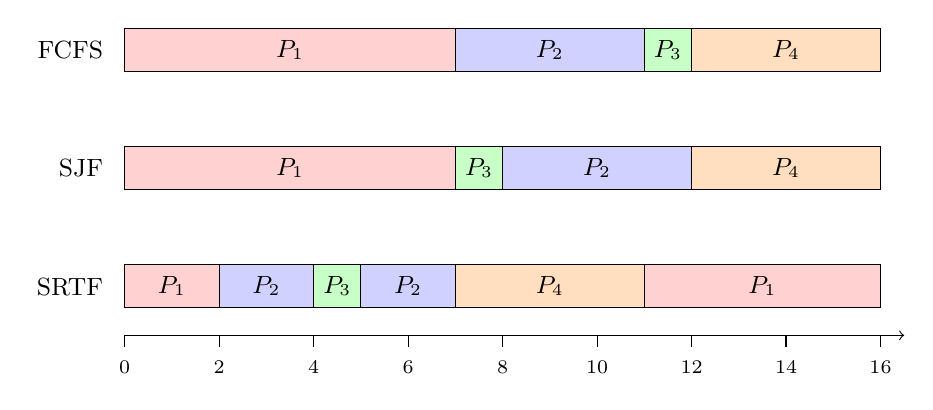
\begin{tikzpicture}[font=\small]
    \def\s{0.6}
    % ---- FCFS ----
    \node[anchor=east] at (-0.15,3.27) {FCFS};
    \draw[fill=red!18] (0,3.0) rectangle ({7*\s},3.55);
    \node at ({3.5*\s},3.275) {$P_1$};
    \draw[fill=blue!18] ({7*\s},3.0) rectangle ({11*\s},3.55);
    \node at ({9*\s},3.275) {$P_2$};
    \draw[fill=green!22] ({11*\s},3.0) rectangle ({12*\s},3.55);
    \node at ({11.5*\s},3.275) {$P_3$};
    \draw[fill=orange!25] ({12*\s},3.0) rectangle ({16*\s},3.55);
    \node at ({14*\s},3.275) {$P_4$};
    % ---- SJF ----
    \node[anchor=east] at (-0.15,1.77) {SJF};
    \draw[fill=red!18] (0,1.5) rectangle ({7*\s},2.05);
    \node at ({3.5*\s},1.775) {$P_1$};
    \draw[fill=green!22] ({7*\s},1.5) rectangle ({8*\s},2.05);
    \node at ({7.5*\s},1.775) {$P_3$};
    \draw[fill=blue!18] ({8*\s},1.5) rectangle ({12*\s},2.05);
    \node at ({10*\s},1.775) {$P_2$};
    \draw[fill=orange!25] ({12*\s},1.5) rectangle ({16*\s},2.05);
    \node at ({14*\s},1.775) {$P_4$};
    % ---- SRTF ----
    \node[anchor=east] at (-0.15,0.27) {SRTF};
    \draw[fill=red!18] (0,0) rectangle ({2*\s},0.55);
    \node at ({1*\s},0.275) {$P_1$};
    \draw[fill=blue!18] ({2*\s},0) rectangle ({4*\s},0.55);
    \node at ({3*\s},0.275) {$P_2$};
    \draw[fill=green!22] ({4*\s},0) rectangle ({5*\s},0.55);
    \node at ({4.5*\s},0.275) {$P_3$};
    \draw[fill=blue!18] ({5*\s},0) rectangle ({7*\s},0.55);
    \node at ({6*\s},0.275) {$P_2$};
    \draw[fill=orange!25] ({7*\s},0) rectangle ({11*\s},0.55);
    \node at ({9*\s},0.275) {$P_4$};
    \draw[fill=red!18] ({11*\s},0) rectangle ({16*\s},0.55);
    \node at ({13.5*\s},0.275) {$P_1$};
    % ---- 时间轴 ----
    \draw[->] (0,-0.35) -- ({16*\s+0.3},-0.35);
    \foreach \x in {0,2,4,6,8,10,12,14,16} {
        \draw (\x*\s,-0.35) -- (\x*\s,-0.5);
        \node[font=\scriptsize] at (\x*\s,-0.75) {\x};
    }
\end{tikzpicture}
\caption{FCFS / SJF / SRTF 甘特图（同一进程集合，时间单位）}
\end{figure}

\begin{table}[H]
\centering
\caption{三种非交互算法对比}
\begin{tabulary}{\textwidth}{CCCC}
\toprule
算法 & 抢占 & 平均周转 & 平均等待 \\
\midrule
FCFS & 否 & 8.75 & 4.75 \\
SJF  & 否 & 8.00 & 4.00 \\
SRTF & 是 & 7.00 & 3.00 \\
\bottomrule
\end{tabulary}
\end{table}

\noindent SRTF 的指标最好，但抢占带来更多上下文切换；且三者都以「长作业饥饿」为代价换取短作业的响应。SJF/SRTF 的理论最优性依赖运行时间可预知，实际系统只能用历史行为估计。

\section{时间片轮转 RR 与优先级调度}

\subsection{时间片轮转 RR}

RR 为每个进程分配一个固定时间片 $q$，就绪队列按 \textbf{FIFO 轮转}：进程用完一个时间片即被抢占并排到队尾；若在时间片内完成或主动阻塞则提前让出。RR \textbf{抢占}且天然公平，是分时系统的基石。

取与上表相同运行时间但\textbf{同时到达}的进程，$q=2$：序列为
\[
P_1[0,2] \to P_2[2,4] \to P_3[4,5] \to P_4[5,7] \to P_1[7,9] \to P_2[9,11] \to P_4[11,13] \to P_1[13,16]
\]
完成时刻 $c=(16,11,5,13)$，于是
\begin{equation}
    \overline{T_{\text{周转}}} = \frac{16+11+5+13}{4} = 11.25,\qquad
    \overline{T_{\text{等待}}} = \frac{9+7+4+9}{4} = 7.25,\qquad
    \overline{T_{\text{响应}}} = \frac{0+2+4+5}{4} = 2.75
\end{equation}

\begin{figure}[H]
\centering
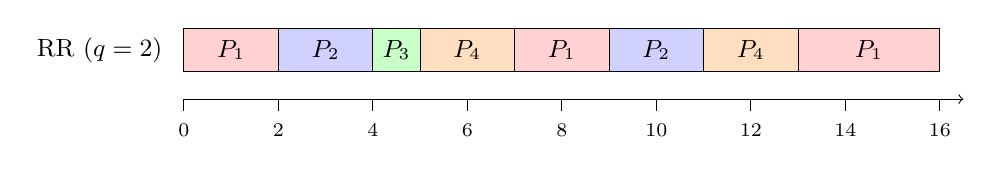
\begin{tikzpicture}[font=\small]
    \def\s{0.6}
    \node[anchor=east] at (-0.15,1.27) {RR ($q=2$)};
    \draw[fill=red!18] (0,1.0) rectangle ({2*\s},1.55);
    \node at ({1*\s},1.275) {$P_1$};
    \draw[fill=blue!18] ({2*\s},1.0) rectangle ({4*\s},1.55);
    \node at ({3*\s},1.275) {$P_2$};
    \draw[fill=green!22] ({4*\s},1.0) rectangle ({5*\s},1.55);
    \node at ({4.5*\s},1.275) {$P_3$};
    \draw[fill=orange!25] ({5*\s},1.0) rectangle ({7*\s},1.55);
    \node at ({6*\s},1.275) {$P_4$};
    \draw[fill=red!18] ({7*\s},1.0) rectangle ({9*\s},1.55);
    \node at ({8*\s},1.275) {$P_1$};
    \draw[fill=blue!18] ({9*\s},1.0) rectangle ({11*\s},1.55);
    \node at ({10*\s},1.275) {$P_2$};
    \draw[fill=orange!25] ({11*\s},1.0) rectangle ({13*\s},1.55);
    \node at ({12*\s},1.275) {$P_4$};
    \draw[fill=red!18] ({13*\s},1.0) rectangle ({16*\s},1.55);
    \node at ({14.5*\s},1.275) {$P_1$};
    \draw[->] (0,0.65) -- ({16*\s+0.3},0.65);
    \foreach \x in {0,2,4,6,8,10,12,14,16} {
        \draw (\x*\s,0.65) -- (\x*\s,0.5);
        \node[font=\scriptsize] at (\x*\s,0.25) {\x};
    }
\end{tikzpicture}
\caption{RR 甘特图（时间片 $q=2$，进程同时到达）}
\end{figure}

\subsection{时间片大小的影响}

时间片 $q$ 是 RR 最重要的参数，直接决定「响应性」与「切换开销」的折中：

\begin{itemize}
    \item $q \to \infty$：RR 退化为 FCFS，响应时间变差，但切换最少。
    \item $q \to 0$：每个指令都切换，上下文切换开销吞掉有效计算，吞吐量骤降。
    \item $q$ 应略大于「一次上下文切换时间」且覆盖绝大多数 CPU 突发，经验上取 $10\sim100$ ms。
\end{itemize}

对同一集合（同时到达）计算不同 $q$（切换开销忽略）：

\begin{table}[H]
\centering
\caption{时间片 $q$ 对指标的影响（同时到达）}
\begin{tabulary}{\textwidth}{CCCC}
\toprule
时间片 $q$ & 平均等待 & 平均响应 & 平均周转 \\
\midrule
1 & 7.00 & 1.50 & 11.00 \\
2 & 7.25 & 2.75 & 11.25 \\
4 & 7.50 & 5.25 & 11.50 \\
$\infty$ (FCFS) & 7.50 & 7.50 & 11.50 \\
\bottomrule
\end{tabulary}
\end{table}

\noindent 结论：在上例中总完成时间恒为 16（单 CPU、不空闲），但\textbf{时间片越小，响应越快}（首轮轮转更早到达每个进程），代价是切换更频繁；时间片越大越接近 FCFS。因此 $q$ 的选取要在响应时间与吞吐量之间折中。

\subsection{优先级调度}

每个进程赋予一个优先级，调度器总是选择\textbf{优先级最高}的就绪进程。约定数值越小优先级越高。优先级可\textbf{静态}给定，也可\textbf{动态}调整。主要问题有二：

\begin{itemize}
    \item \textbf{饥饿 (starvation)}：低优先级进程可能长期得不到 CPU。
    \item \textbf{优先级反转 (priority inversion)}：低优先级进程持有高优先级进程所需的锁，导致后者被中优先级进程阻塞，可用优先级继承缓解。
\end{itemize}

对同时到达、优先级为 $P_2(1)>P_4(2)>P_1(3)>P_3(4)$ 的集合做非抢占优先级调度，序列为
\[
P_2[0,4] \to P_4[4,8] \to P_1[8,15] \to P_3[15,16]
\]
\begin{equation}
    \overline{T_{\text{周转}}} = \frac{15+4+16+8}{4} = 10.75,\qquad
    \overline{T_{\text{等待}}} = \frac{8+0+15+4}{4} = 6.75
\end{equation}

\begin{figure}[H]
\centering
\begin{tikzpicture}[font=\small]
    \def\s{0.6}
    \node[anchor=east] at (-0.15,0.27) {优先级};
    \draw[fill=blue!18] (0,0) rectangle ({4*\s},0.55);
    \node at ({2*\s},0.275) {$P_2$};
    \draw[fill=orange!25] ({4*\s},0) rectangle ({8*\s},0.55);
    \node at ({6*\s},0.275) {$P_4$};
    \draw[fill=red!18] ({8*\s},0) rectangle ({15*\s},0.55);
    \node at ({11.5*\s},0.275) {$P_1$};
    \draw[fill=green!22] ({15*\s},0) rectangle ({16*\s},0.55);
    \node at ({15.5*\s},0.275) {$P_3$};
    \draw[->] (0,-0.35) -- ({16*\s+0.3},-0.35);
    \foreach \x in {0,2,4,6,8,10,12,14,16} {
        \draw (\x*\s,-0.35) -- (\x*\s,-0.5);
        \node[font=\scriptsize] at (\x*\s,-0.75) {\x};
    }
\end{tikzpicture}
\caption{非抢占优先级调度甘特图（数值小者优先）}
\end{figure}

\noindent RR 与优先级的结合即\textbf{优先级 + 时间片}：高优先级队列内轮转，既保响应又防独占。

\section{多级反馈队列 MLFQ}

MLFQ 不要求预知运行时间，而是用「多个优先级队列 + 反馈」动态推测进程类型（CPU 密集型还是 I/O 密集型）。核心规则：

\begin{enumerate}
    \item \textbf{多队列、优先级递减}：设 $Q_0,Q_1,\dots,Q_{n-1}$，$Q_0$ 优先级最高。总是调度最高优先级非空队列中的进程。
    \item \textbf{时间片随层级递增}：高优先级队列用短时间片（如 $Q_0$ 为 2），低优先级队列用长时间片（如 $Q_1$ 为 4，$Q_2$ 为 FCFS），以适配不同进程。
    \item \textbf{新进程入最高队列}：所有新进程先进入 $Q_0$，享受最短响应。
    \item \textbf{用完整个时间片则降级}：进程若耗尽分配的整个时间片仍未完成，说明偏 CPU 密集，被降到下一级队列。
    \item \textbf{主动让出则保持/升级}：进程在时间片用完前主动让出（如等待 I/O），说明偏交互式，留在原队列（或提升），从而持续获得好响应。
    \item \textbf{周期提升 (priority boost)}：每隔固定时间 $S$，把所有进程重新提到 $Q_0$，防止长作业饥饿，并校正对 CPU/IO 类型的误判。
    \item \textbf{同队列内轮转}：同一优先级队列内部按 RR 调度。
\end{enumerate}

\begin{table}[H]
\centering
\caption{MLFQ 队列参数（示例）}
\begin{tabulary}{\textwidth}{CCCC}
\toprule
队列 & 优先级 & 时间片 & 典型对象 \\
\midrule
$Q_0$ & 最高 & 2 & 新进程、交互式 (I/O 密集) \\
$Q_1$ & 中 & 4 & 短批处理 \\
$Q_2$ & 最低 & FCFS & CPU 密集型长作业 \\
\bottomrule
\end{tabulary}
\end{table}

\noindent MLFQ 用「降级惩罚 CPU 密集、保留奖励 I/O 密集、周期提升兜底饥饿」三条机制，在无需预知运行时间的前提下同时兼顾响应时间与吞吐量，是通用操作系统最常用的调度框架之一。
